\section{Lösungsansatz}
\label{sec-4}

Nachdem in den vorangegangenen Kapiteln die Hintergründe erläutert und Probleme identifiziert wurden, beschreibt dieses Kapitel nun einen möglichen Lösungsansatz. Die Idee baut auf dem Ansatz von Strzys et. al. auf und soll zunächst in ihren Grundzügen dargestellt und konkretisiert werden.

\subsection{Designentscheidungen bezüglich der AR-Umgebung}
\label{sec-4-1}
Im Kern besteht der Ansatz darin, die physikalischen Eigenschaften darzustellen, in ihren realen Kontext einzubetten und dadurch einen räumlichen und zeitlichen Zusammenhang zu schaffen. Die Versuchsaufbauten werden mit virtuellen Objekten angereichert und somit in eine gemeinsame Anwendung integriert. Die Nutzererfahrung entsteht also durch das Zusammenspiel von realer und virtueller Welt.\\

Das bedeutet also, dass die virtuellen Objekte in Relation zum Versuchsaufbau, vor allem zur Spule, platziert werden. Das betrifft vor allem die Darstellungen der Magnetfelder. Dementsprechend muss die genaue Position und Ausrichtung relevanter Geräte bestimmt und in das Koordinatensystem der Anwendung transformiert werden. Nachdem dies einmal erfolgt ist, muss der Vorgang im Laufe der Anwendung nicht wiederholt werden, denn der Aufbau wird im Laufe des Versuches nicht bewegt oder gedreht. Der Anwender kann sich dann frei um die Gerätschaften herum bewegen, sie aus verschiedenen Perspektiven betrachten und damit interagieren. Die Interaktion erfolgt dabei sowohl mit den realen als auch den virtuellen Objekten.\\

Neben dem räumlichen Zusammenhang wird auch ein zeitlicher hergestellt. Dies geschieht, indem die Brille in Echtzeit Messwerte von Geräten des Versuches erhält. Diese werden dann verarbeitet und dazu in Zusammenhang stehende Darstellungen angepasst. Das betrifft in erster Linie die Visualisierungen des Magnetfeldes der Spule, die sich automatisch an die gemessenen Werte anpassen. Das bedeutet, dass der Nutzer beim Einstellen des Stromflusses an der Spannungsquelle die Änderungen an den physikalischen Eigenschaften gleichsam in der Realität als auch der virtuellen Realität in Echtzeit beobachten kann. \\

Dieses Konzept macht dabei von den zentralen Stärken der HoloLens Gebrauch. Als Head Mounted Display mit transparenter, stereoskopischer Anzeige und dem Raumverständnis sind solch immersive Anwendungsszenarien die Kernkompetenz der Brille. Dazu trägt auch die Bewegungsfreiheit sowie der Punkt, dass der Träger die Hände frei hat, bei.

\vspace{8px}
\begin{center}
	\fbox{
		\parbox{0.9\linewidth}{
		\vspace{4px}
		\textbf{Überblick}
		\begin{itemize}[rightmargin=12px, topsep=-12px]
			\setlength{\itemsep}{-1pt}
			\singlespacing
			\item Integration von realen und virtuellen Objekten in eine Mixed Reality Anwendung
			\item Virtuelle Objekte werden in den Versuchsaufbau eingebettet und interagieren mit diesem in Echtzeit
			\item Gemessene, berechnete und beobachtete physikalische Vorgänge werden somit in einer Anwendung integriert
			\item Nutzer kann sich mit der HoloLens frei im Raum bewegen und mit der Anwendung sowie den Gerätschaften interagieren
			\item Zentral ist dabei die Darstellung der entstehenden Magnetfelder
		\end{itemize}
	\vspace{18px}
	}}\\
\end{center}
\vspace{6px}


Unter diesem grundsätzlichen Ansatz soll die Lösung nun weiter konkretisiert werden. Dazu erläutert die Arbeit zunächst das Design der Darstellungen und darauf folgend die Interaktion und Steuerung der Anwendung. Das Kapitel schließt mit einer kurzen Zusammenfassung des Designs.

\subsection{Designentscheidungen bezogen auf HoloLens}
\label{sec-4-2}
Viele Darstellungen sollen am Versuchsaufbau, also vor allem an der Spule, verankert werden. Das bedeutet, dass der Anwender Abstand und Blickwinkel zu diesen Objekten durch seine Bewegungen und Blickrichtung selbst steuert. Um dennoch stets eine komfortable Nutzung zu ermöglichen, und die zuvor erläuterten Probleme im Hinblick auf Distanz und Blickrichtung zu vermeiden, werden mehrere Maßnahmen getroffen.\\

\textit{Distanz}\\
Um zu geringe Distanzen zwischen Nutzer und den virtuellen Objekten zu vermeiden, werden fest verankerte Darstellung unterhalb einer gewissen Distanz ausgeblendet. Hier folgt das Design den entsprechenden, zuvor aufgeführten Empfehlungen. Das ermöglicht dem Nutzer zugleich das Eintauchen in die Darstellungen. Frei bewegliche Elemente hingegen werden durch entsprechende Skripte den Bewegungen des Nutzers angepasst, so dass sie stets in einer komfortablen Zone des Sichtfeldes verbleiben.\\

Weiterhin soll eine Nutzung im Abstand von ca. 1,2m bis 1,5m begünstigt werden. Das hat mehrere Gründe. Zum einen passt bei diesem Abstand die Spule vollständig in das Sichtfeld der HoloLens. Darin eingebettete Darstellungen werden also nicht durch die Grenzen des Field of View abgeschnitten. Dabei bleibt auch noch etwas Spielraum für Kopfbewegungen, so dass die Darstellungen nicht schon bei kleinen Bewegungen an die Grenzen des Displays stoßen. Gleichzeitig bleiben nicht so große Teile des Sichtfeldes ungenutzt. Außerdem reduzieren sich so die Effekte durch die Diskrepanz zwischen Konvergenz und Akkommodation der Augen im Vergleich zu kleineren Abständen. Hier findet also ein Kompromiss zwischen Ausnutzung des Sichtfeldes und Komfort statt. Der genannte Bereich wurde dabei aus praktischer Erfahrung festgelegt.\\

\textit{Größe \& Blickrichtung}\\
Für die Darstellungen bedeutet das, dass die Größe der Objekte für diesen Bereich geeignet sein sollte. Darüber hinaus kann die Auswahl eines geeigneten Tisches die Nutzung begünstigen. Das Design geht davon aus, dass der Nutzer die Anwendung im Stehen verwendet, damit er in der Lage ist, sich frei um den Versuchsaufbau herum zu bewegen. Ein entsprechend hoher Tisch führt dazu, dass der vertikale Blickwinkel im empfohlenen Bereich zwischen 0° und 35° unterhalb der Horizontlinie liegt. Weiterhin kann die Spule mit etwas Abstand zur Tischkante positioniert werden, um so auf natürliche Weise die Nutzung in der geeigneten Distanz zu begünstigen.\\

\textit{Begrenzungen durch FOV und Auflösung}\\
HL begrenzte Auflösung und Sichtfeld. Lösungsansatz verfolgt daher Strategie, visuellen Clutter zu vermeiden. \\

\textit{Farbe}

\subsection{Designentscheidungen bezogen auf Infos}
Warum wird was dargestellt????
\begin{itemize}
	\item Strukturelle Eigenschaften (Stärke, Richtung, Homogenität) des Magnetfeldes im Inneren der Spule sind grundlegend zum Verständnis des Versuches. MFeld 3D darstellen. Beide Darstellungsmodelle anbieten. 
\end{itemize}
\subsection{Wie erfolgt die Darstellung?}
Weiterhin sind für alle Objekte, die in Abhängigkeit des sich ändernden Feldes stehen, Parameter für die Darstellung definiert. Diese legen für alle Elemente einen gemeinsamen Wertebereich fest, für den die Darstellung erfolgt. Außerdem werden ab dem minimalen Wert die Objekte über einen gewählten Bereich kontinuierlich eingeblendet. Dieses konsistente Verhalten dient dazu, das Verständnis der Darstellungen zu verbessern. Außerdem soll auf diese Weise transportiert werden, dass nur die Darstellungen verschwinden, nicht jedoch die physikalischen Sachverhalte, die repräsentiert werden.\\
\subsubsection{Das Magnetfeld}
\label{sec-4-2-2}
Die Darstellung des Magnetfeldes von Erde und Spule ist zentraler Bestandteil der Anwendung.

\textit{Visuelle Gestaltung}\\
Die Darstellung des Feldes erfolgt über 3D-Pfeile bzw. -Pfeillinien. Diese werden schattiert, damit die Form und Ausrichtung im Raum besser erkennbar wird. Beide verwenden dafür den gleichen Shader. Die Größe der Objekte wurde anhand von Erfahrungswerten angepasst. Durchmesser und Länge sind vergleichbar mit denen eines Kugelschreibers oder dickeren Stiftes. Als Farben wurden Hellblau und Orange für den Anteil der Spule bzw. der Erde gewählt. Blau wird oft für Magnetfeldlinien verwendet und wird daher auch hier gebraucht. Allerdings wird ein weniger gesättigtes, helleres Blau verwendet, damit die Deckkraft vor helleren Hintergründen nicht verloren geht. Das Orange weißt die selbe Sättigung und Helligkeit auf wie das Blau, damit sich die Objekte nicht in der Transparenz voneinander unterscheiden.\\

\textit{Begrenzung der Darstellung}\\
Die Visualisierung des Feldes erfordert die Festlegung eines darzustellenden Bereiches für die Flussdichte. Ein Intervall lässt sich in der Anwendung frei über die Einstellungen festlegen. Diese Einstellungsmöglichkeit ist für die praktische Nutzung wesentlich, da die gemessene Flussdichte des Erdmagnetfeldes in Abhängigkeit von der Umgebung variieren kann. Voreingestellt ist ein Bereich von $3\mu T$ bis $60\mu T$, die Flussdichte der Erde liegt mit $30 \mu T$ bis $40 \mu T$ im mittleren Bereich dieser Skala. Am unteren Ende des Bereiches werden die Objekte über Transparenz ausgeblendet.\\

Nach oben hin ist keine Darstellung der Begrenzung vorgesehen. Der Bereich sollte so gewählt werden, dass die obere Grenze durch die maximal am Regler einstellbare Stromstärke nicht erreicht werden kann. Somit erfährt der Anwender die Limitierung der Darstellung auf natürliche Weise. Die Konfiguration der Schaltung kann hier über eingebaute Widerstände so an die Spannungsquelle angepasst werden, dass der erzeugte Stromfluss im gewünschten Bereich liegt.\\

\begin{comment}

\begin{figure}[h!]
\centering
\includegraphics[width=0.8\textwidth]{images/todo.jpg}
\caption{Magnetfeld Design}
\label{img:magnetic-design}
\end{figure}
\end{comment}

\vspace{8px}
\begin{center}
	\fbox{
		\parbox{0.9\linewidth}{
			\vspace{4px}
			\textbf{Überblick}
			\begin{itemize}[rightmargin=12px, topsep=-12px]
				\setlength{\itemsep}{-1pt}
				\singlespacing
				\item Magnetfeld von Erde und Spule über 3D-Geometrie darstellen und räumlich in die Spule einbetten
				\item Einbettung durch Verdeckungsberechnung von realer Spule und virtueller Geometrie verbessern	
				\item Komponenten des Feldes (Erde, Spule) mit verschiedenen Farben darstellen anstelle des tatsächlichen, kombinierten Feldes
				\item Sowohl die Darstellung über Feldlinien als auch die über Vektoren anbieten, Nutzer kann zwischen den Varianten umschalten
				\item Darstellung beschränkt sich auf einen zylindrischen Ausschnitt der Spule	
				\item Objekte verändern sich dynamisch anhand von Messwerten
				\item Eine davon unabhängige, eigene Darstellung von Simulationsdaten zeigt eine numerische Lösung für das Feld sowohl innerhalb als auch außerhalb der Spule für eine ausgewählte Ebene
			\end{itemize}
			\vspace{18px}
	}}\\
\end{center}
\vspace{6px}

\textit{3D-Objekte}\\
Die Repräsentation über dreidimensionale Objekte erlaubt die Betrachtung aus beliebigen Blickwinkeln. Zweidimensionale Linien oder Pfeile würden hier dazu führen, dass die Darstellung beim Blick in Richtung des Feldstärkevektors verschwindet. Außerdem stärkt ein 3D-Objekt das Präsenzgefühl und unterstützt so die Glaubhaftigkeit der Einbettung. Letztere wird dabei vor allem durch die Verdeckung der Feldlinien und Vektoren durch die Spule unterstützt. Die Überdeckung von weiter entfernten Objekten durch nähergelegende ist einer der wichtigsten Faktoren für die menschliche Tiefenwahrnehmung und ist hier daher unverzichtbar.\\

\textit{Komponenten des Feldes}\\
Die Entscheidung, die einzelnen Komponenten des Feldes mit verschiedenen Farben darzustellen anstelle des tatsächlichen, überlagerten Feldes, wurde aus didaktischen Gründen getroffen. Für das Verständnis, wie das resultierende Feld entsteht, ist die Visualisierung der Komponenten entscheidend. Deshalb wurde auf Empfehlung der Didaktiker diese Variante gewählt. Damit jedoch nicht der falsche Eindruck entsteht, es würden sich um zwei unabhängige, eigene Magnetfelder handeln, sollte der Anwender darüber informiert werden. Dies kann z.B. durch ein Voice Over mit einem kurzen Erklärtext oder auch eine Fachkundige Person, z.B. eine Lehrkraft, erfolgen.\\

\textit{Modelle und Begrenzung}\\
Weiterhin werden die beiden, in der Lehre üblichen Darstellungsmodelle angeboten. Beide Modelle bringen Vor- und Nachteile mit sich. Der Nutzer kann im Laufe der Anwendung frei zwischen den Modellen wechseln. Dadurch können beide Modelle ihre individuellen Stärken ausspielen. Außerdem ist so ein besseres Verständnis davon möglich, wie die Modelle zusammenhängen.\\

Beide Modelle beschränken sich zunächst auf einen zylindrischen Ausschnitt der Spule. Das ist ausreichend, da für den Versuch lediglich das Feld im Zentrum der Spule, in dem sich auch der Kompass befindet, relevant ist. Das inhomogene Feld außerhalb der Spule wirkt sich nicht auf den Versuch aus. Dies wird daher in einer eigenen Darstellung auf Basis von vorberechneten Simulationsdaten dargestellt. So wird zum einen vermittelt, wie das gesamte Feld aussieht, und zum anderen, warum der Kompass gerade in die Mitte der Spule gestellt wird.\\

Die Darstellungen verändern sich dabei dynamisch, entsprechend ihrer Modelle, anhand der aus den Messwerten berechneten Flussdichte. Beim Feldlinienmodell verändern sich Anzahl, Position und Abstand der Linien, bei den Vektoren variiert die Länge. Für die Flussdichte des Erdmagnetfeldes wird ein zuvor gemessener Wert angenommen.\\

\textbf{Vektoren}\\
Die Umsetzung der Vektordarstellung ist in Abb. \ref{img:mfield-vectors} näher zu sehen.
\begin{figure}[H]
	\centering
	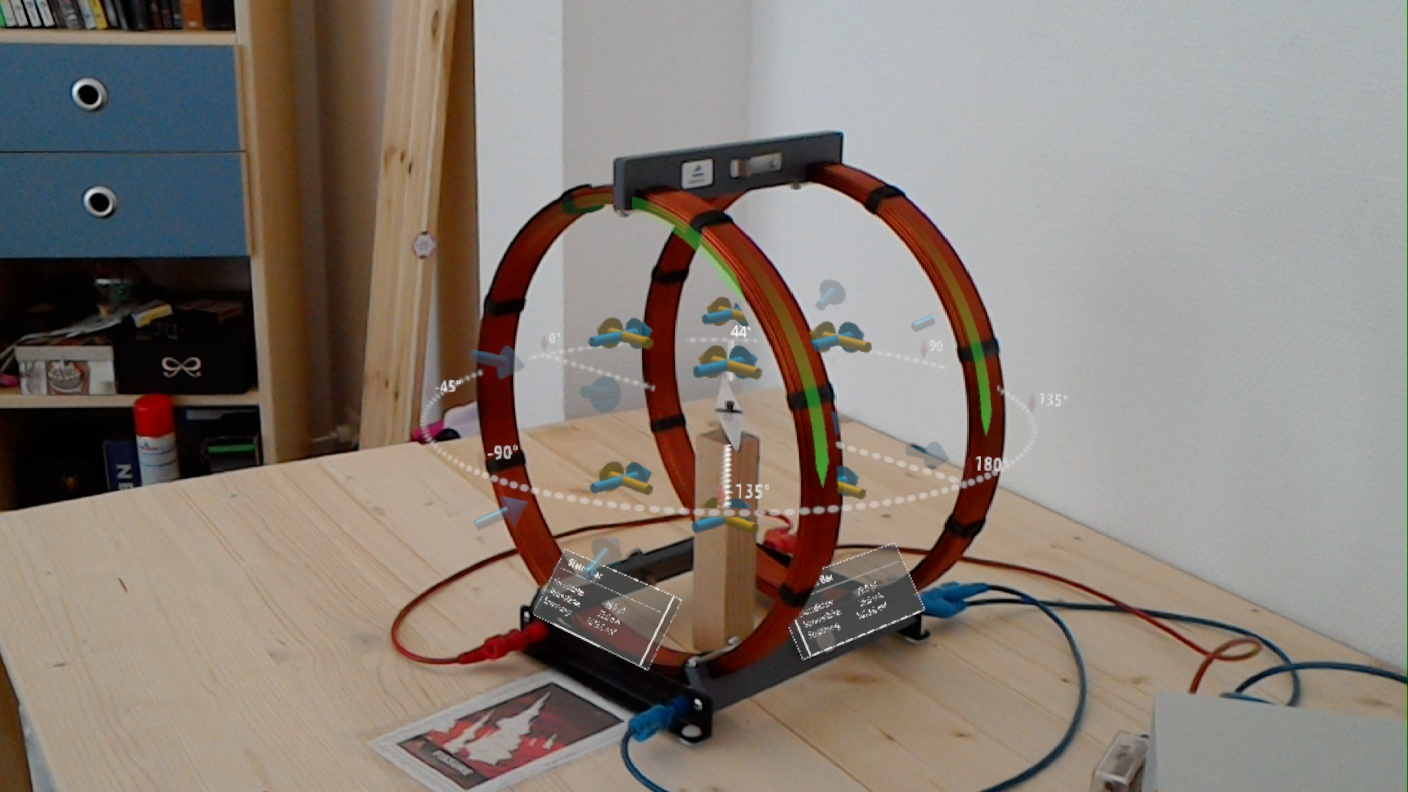
\includegraphics[width=0.8\textwidth]{images/HL/vectors.jpg}
	\caption{Vektoren}
	\label{img:mfield-vectors}
\end{figure}
\vspace{4px}
\begin{center}
	\fbox{
		\parbox{0.9\linewidth}{
			\vspace{4px}
			\textit{Überblick}
			\begin{itemize}[rightmargin=12px, topsep=-12px]
				\setlength{\itemsep}{-1pt}
				\singlespacing
				\item Pfeile repräsentieren Feldstärkevektor über Länge und Ausrichtung
				\item 8 Pfeile für homogenes Feld, weitere 8 für Andeutung inhomogenes Feld
				\item Anordnung im 3D-Gitter mit konfigurierbaren Parametern (Abstand und Anzahl, jeweils pro Raumrichtung)
				\item Ankerpunkt mittig im Pfeil
			\end{itemize}
			\vspace{18px}
	}}\\
\end{center}
\vspace{6px}

\textit{Anordnung und Anzahl}\\
In der Vektordarstellung werden mindestens acht Vektoren benötigt, damit die zuvor genannten Eigenschaften erkennbar werden. Dabei gelten die gleichen Gründe wie zuvor. Während jedoch eine Feldlinie das Feld in Richtung der Z-Achse kontinuierlich darstellt, sind hier wenigstens zwei Vektoren notwendig. Die Anordnung erfolgt in einem 3D-Gitter, bei dem die Anzahl und die Abstände pro Dimension parametrisiert sind. Auch hier gilt, dass mehr Objekte im homogenen Teil des Feldes keine weiteren Informationen transportieren. Daher wurde in Anbetracht des zur Verfügung stehenden Raumes in die Größe anstelle der Anzahl der Objekte investiert.\\

\textit{Skalierung}\\
Die Flussdichte wird im Fall der Pfeile über deren Länge und Richtung ausgedrückt. Die Form der Objekte soll mit einer sich ändernden Länge nicht verzerrt werden. Eine einfache Skalierung der Pfeillänge würde jedoch dazu führen, dass auch die Pfeilspitze in die Länge gezogen wird. Daher wird die Geometrie zur Laufzeit angepasst und nur ein Teil in der Mitte verändert.\\

\textit{Bezugspunkt}\\
Welcher Punkt dem Vektor als Ankerpunkt dient ist dabei nicht entscheidend, denn ein Pfeil repräsentiert jeden Punkt des homogenen Feldes. Eine explizite Darstellung ist daher nicht erforderlich. Allerdings wird die Verankerung im Mittelpunkt dadurch deutlich, dass die Position bei variierender Länge gleich bleibt.\\

\textit{Inhomogener Anteil}\\
Im Gegensatz zu den Feldlinien ist eine Darstellung des inhomogenen Feldes über Vektoren auch ohne aufwendige Echtzeit-Berechnungen möglich (siehe Kap. \ref{sec-2-2-2}). Die Anwendung nutzt diese Eigenschaft, um in dieser Darstellung auch das inhomogene Feld anzudeuten. Dies geschieht, indem das Raster so gewählt wird, dass vor und hinter der Spule (im Sinne der Z-Achse) jeweils eine Reihe Vektoren positioniert ist. Diese sind hier im Vergleich deutlich kürzer und nicht parallel, sondern nach innen bzw. nach außen gerichtet. So wird erkennbar, dass das Feld hier schwächer und inhomogen ist. Da die Darstellungen erst ab einem minimalen Wert eingeblendet werden, wird der inhomogene Teil nach dem homogenen Teil eingeblendet.\\



\subsubsection{Der Stromfluss} 
\label{sec-4-2-3}
Beim Stromfluss ist in erster Linie die Flussrichtung durch die Spulen von Interesse, denn hiervon hängt die Ausrichtung des entstehenden Magnetfeldes ab. Diese wird über pfeil-ähnliche Indikatoren an den Spulen angezeigt. Außerdem werden die Anschlüsse mit Labels versehen, die Plus und Minus kennzeichnen.

\begin{comment}
Das Konzept ist in Grafik \ref{img:current-design} dargestellt.

\begin{figure}[h!]
\centering
\includegraphics[width=0.8\textwidth]{images/todo.jpg}
\caption{Stromfluss Design}
\label{img:current-design}
\end{figure}
\end{comment}

\vspace{8px}
\begin{center}
	\fbox{
		\parbox{0.9\linewidth}{
			\vspace{4px}
			\textbf{Überblick}
			\begin{itemize}[rightmargin=12px, topsep=-12px]
				\setlength{\itemsep}{-1pt}
				\singlespacing
				\item Direkt an den Spulen verankerte Indikatoren zeigen die Flussrichtung an
				\item Indikatoren passen sich der Position des Nutzers an
				\item Kennzeichnung der Konnektoren mit Plus und Minus anhand von Labels
			\end{itemize}
			\vspace{18px}
	}}\\
\end{center}
\vspace{6px}
\textit{Positionierung und Ausrichtung}\\
Die Indikatoren werden abhängig von Position und Blickwinkel des Betrachters angezeigt, wie in der Abbildung zu sehen. Auf diese Weise ist die Richtung aus allen Perspektiven zu erkennen. Beim Wechsel der Darstellungen gibt es einen kontinuierlichen Übergang. In dieser Umsetzung ist die 2D-Geometrie ausreichend. Die Positionierung direkt auf bzw. an den Spulen führt dazu, dass kein zusätzlicher Screenspace, der für die Felddarstellung genutzt wird, in Anspruch genommen werden muss, da das Feld hier ohnehin von den Spulen verdeckt wird. Die Spulen bleiben weiterhin gut sichtbar, da nur ein Teil und nur eine Seite überdeckt wird. Hier haushaltet die Anwendung also mit dem ihr zur Verfügung stehenden Platz.\\

Ein Nachteil dieser Lösung ist jedoch, dass das zuvor erläuterte Problem mit der Akkommodation auftritt. Die Kante zwischen virtuellem Pfeil und realer Spule kann bei einer Entfernung unter 2m zu Irritationen führen, da sich das Auge auf eine Akkommodation festlegen muss und dementsprechend das andere Objekt nicht als scharf wahrnimmt. Allerdings stehen beide Objekte selten im Fokus und die Spule muss nicht detailreich betrachtet werden, deshalb überwiegen hier die Vorteile dieser Lösung.\\

\textit{Annotationen der Anschlüsse}\\
Damit die Stromrichtung auch als technische Stromrichtung interpretiert und in die Schaltung eingeordnet werden kann, sind die Konnektoren mit Labels in Form von Tooltips mit Bezeichnung, entsprechender Farbe und Icon ausgestattet. Die Lables orientieren sich dabei an der Kamera, damit sie aus allen Winkeln lesbar sind.\\

\subsubsection{Der Kompass} 
\label{sec-4-2-4}
Der Kompass bildet sich aus dem Zusammenspiel einer realen Magnetnadel, einer virtuellen Skala sowie virtuellen Hilfslinien. 

\begin{comment}
Die Idee ist in Abbildung \ref{img:compass-design} festgehalten.

\begin{figure}[h!]
\centering
\includegraphics[width=0.8\textwidth]{images/todo.jpg}
\caption{Kompass Design}
\label{img:compass-design}
\end{figure}
\end{comment}

\vspace{8px}
\begin{center}
	\fbox{
		\parbox{0.9\linewidth}{
			\vspace{4px}
			\textbf{Überblick}
			\begin{itemize}[rightmargin=12px, topsep=-12px]
				\setlength{\itemsep}{-1pt}
				\singlespacing
				\item Kompass entsteht aus Kombination von realer Magnetnadel und virtueller Skala
				\item Reale Nadel wird mittig in der Spule aufgestellt
				\item Virtueller Ring mit Markierungen im 45° Abstand um die Spule herum dient als Skala	
				\item Virtuelle Kreissehnen durch den Mittelpunkt mit Ausschnitt im Mittelpunkt für den Kompass 
				\begin{itemize}[topsep=0px, label=\textbullet]
					\setlength{\itemsep}{-1pt}
					\item Feste Nord-Süd Linie
					\item Feste 45° Linie
					\item Virtueller Kompass, der die theoretisch berechnete Auslenkung eines idealen Kompasses anzeigt
				\end{itemize}
				\item Gradzahl der theoretischen Nadel wird am Kreis angezeigt
			\end{itemize}
			\vspace{18px}
	}}\\
\end{center}
\vspace{6px}

Der Fokus dieses Designs liegt nicht darin, die Auslenkung des Kompasses möglichst genau ablesen zu können. Vielmehr geht es darum die besonders wichtigen Auslenkungen, nämlich 0° und 45°, sichtbar zu machen. Denn Ziel des Versuches ist es, die Nadel von 0° auf 45° auszulenken. Zwischen diesen Werten genügt eine grobe Orientierung. Außerdem sollen die theoretischen Werte mit in den Kompass integriert werden.\\

Die Nutzung einer virtuellen Skala erlaubt letzteres auf natürliche Weise. Dazu kommen zwei weitere, wesentliche Gründe, warum nicht eine reale Skala zum Einsatz kommt. Erstens wäre eine herkömmliche, unter der Nadel angebrachte Skala nur schwer lesbar. Das liegt an der gewünschten Entfernung, da hierfür die Skalen oft zu klein sind, aber auch am Blickwinkel. Letzterer ist viel geringer als die steilen Winkel, die normalerweise zum Ablesen der Richtung benötigt werden. Die Nadel hingegen ist mit $12 cm$ Länge bewusst groß genug gewählt, damit sie gut zu sehen ist. Zweitens würde sie Platz im inneren der Spule einnehmen. Dieser Platz wird jedoch für die Felddarstellungen benötigt.\\

Die virtuelle Skala umgeht dieses Problem, da sie als Ring unmittelbar außerhalb der Spule umgesetzt ist. Lediglich die Hilfslinien bei 0° und 45° sowie die Linie des virtuellen Kompasses kommen zusätzlich in den Bereich der Felddarstellung. Die ersten beiden werden außerdem etwas abgeschwächt, indem ihre Transparenz erhöht wird. Alle drei sind jedoch in der Mitte ausgeschnitten, um die Kompassnadel nicht zu überblenden.\\

Dieses Design erlaubt es dem Betrachter genau festzustellen, ob die Linie der Nadel durch eine der virtuellen Linien fortgesetzt wird. Außerdem entsteht so die Vergleichbarkeit mit der theoretischen Nadel, da diese entweder stärker, schwächer oder genauso stark ausgelenkt ist. Für letztere wird außerdem die Gradzahl als Text angegeben.\\

Diese Lösung setzt jedoch auf eine genaue Positionsbestimmung der Spule sowie eine hohe Stabilität der Hologramme. Wenn das Modell verrutscht oder zittert schränkt das die Nutzung des Kompasses ein.

\subsubsection{Weitere Informationen} 
\label{sec-4-2-5}
Für die Darstellung weiterer Informationen sind zwei Lösungen vorgesehen: Ein Datenpanel zur Darstellung numerischer Werte in Textform sowie optional aktivierbare Labels am Versuchsaufbau.

\begin{comment}
Beides ist in Abbildung \ref{img:info-design} skizziert.


\begin{figure}[h!]
\centering
\includegraphics[width=0.8\textwidth]{images/todo.jpg}
\caption{Info Design}
\label{img:info-design}
\end{figure}
\end{comment}

\vspace{8px}
\begin{center}
	\fbox{
		\parbox{0.9\linewidth}{
			\vspace{4px}
			\textbf{Überblick}
			\begin{itemize}[rightmargin=12px, topsep=-12px]
				\setlength{\itemsep}{-1pt}
				\singlespacing
				\item Stromstärke (gemessen) und Flussdichte (berechnet) werden auf einem Datenpanel dargestellt
				\item Panel hat einen dunklen Hintergrund, damit der Text besser lesbar ist
				\item Weitere physikalische Parameter werden über Labels an die entsprechenden Elemente angehängt (Windungszahl, Radius und Abstand der Spulen, Widerstand etc.)
			\end{itemize}
			\vspace{18px}
	}}\\
\end{center}
\vspace{6px}

Das Datenpanel dient als Informationsboard für die Echtzeitdaten. Der graue Hintergrund stellt dabei sicher, dass die Schrift gut zu lesen ist. Die Positionierung an den Verbindungsstücken liegt, wie auch bei den Indikatoren für die Stromrichtung, im Ausnutzen von Platz begründet. Hier ist die ständige Sichtbarkeit jedoch sekundär.\\

Man könnte auch eine Lösung über ein Heads-Up Display in Erwägung ziehen, da es sich um numerische Werte handelt, ohne einen natürlichen Ankerpunkt in der Szene. Allerdings sind HUDs aus verschiedenen Gründen auf der HoloLens ungünstig. Deshalb rät die Dokumentation explizit vom Gebrauch solcher ab. Daher wurde hier die Variante eines fest stehenden Objektes gewählt.\\

Schließlich lassen sich verschiedene weitere Parameter des Versuches anzeigen. Diese müssen nicht immer sichtbar sein und können deshalb optional eingeblendet werden. Die Umsetzung erfolgt wie bei den Markierungen für Plus und Minus im Tooltip-Stil.\\
\subsection{Interaktion}
\label{sec-4-4}
Die Interaktion soll möglichst einfach gehalten werden und auch für Nutzer ohne Erfahrung mit der HoloLens geeignet sein. Daher folgt das Design der Empfehlung, alternative Interaktionsmöglichkeiten zur Verfügung zu stellen. Diese Lösung bietet dem Anwender drei Eingabemethoden an:
\begin{enumerate}
	\setlength{\itemsep}{-5pt}
	\item Klicker
	\item Handgesten
	\item Sprachbefehle
\end{enumerate}

\vspace{8px}
\begin{center}
	\fbox{
		\parbox{0.9\linewidth}{
			\vspace{4px}
			\textbf{Überblick}
			\begin{itemize}[rightmargin=12px, topsep=-12px]
				\setlength{\itemsep}{-1pt}
				\singlespacing
				\item Interaktion mittels Klicker, Handgesten und Sprache
				\item Jede Methode kann jederzeit genutzt werden
				\item Visuelles oder akustisches Feedback für Nutzereingaben
				\item Verwendung vorgefertigter, für die HoloLens designeter Objekte
			\end{itemize}
			\vspace{18px}
	}}\\
\end{center}
\vspace{6px}

Der Klicker ist ein kleiner, in der Hand gehaltener Taster, der sich wie eine Maustaste verhält. Ein mal drücken wird als Klick erkannt, aber auch gedrückt halten ist möglich.
Die dazu korrespondierende Handgeste ist der AirTap, der auf der HoloLens als Klick-Geste dient. Als Klick erkennt das Gerät außerdem den reservierten Sprachbefehl ''Select''. Weitere Sprachbefehle werden von der Anwendung selbst definiert.\\

Die Lösung stellt dem Anwender die drei Eingabemethoden frei zur Verfügung. Das bedeutet, der Nutzer kann selbst entscheiden, auf welche Methoden er zurückgreift. Jede Interaktionsmöglichkeit kann jederzeit genutzt werden. Anwender, die keine Erfahrung mit der HoloLens haben, sind nicht gezwungen, zunächst die Gestensteuerung der HoloLens zu erlernen. Außerdem ist die Interaktion so auf natürliche Weise konsistent: Ein Klick mit dem Klicker ist äquivalent zu einem Klick durch den AirTap.\\

\textit{Hauptteil der Anwendung - Durchführung des Versuches}\\
Während der Durchführung des Versuches sind drei Aktionen möglich:
\begin{enumerate}[topsep=-2px]
	\setlength{\itemsep}{-5pt}
	\item Veränderung des Stromflusses über den Regler der Spannungsquelle
	\item Wechsel zwischen den Darstellungsmodellen
	\item Rückkehr zum Hauptmenü
\end{enumerate}
\vspace{8px}

Bei ersterer interagiert der Nutzer mit dem Versuchsaufbau, die Anwendung passt sich dabei automatisch an den sich ändernden Stromfluss anhand der Messwerte an. Für den Wechsel zwischen den Darstellungen sowie die Rückkehr zum Menü werden die zuvor beschriebenen Möglichkeiten angeboten. In jedem Fall reagiert die Anwendung mit visuellem oder akustischem Feedback auf ein Kommando.\\

\textbf{Menü, Einstellungen und Tracking}\\
Das Menü und die Einstellungen werden über Buttons gesteuert. Diese lassen sich über den standardmäßigen Cursor in der Mitte des Sichtfeldes anvisieren und dann mit einem Klick betätigen. Der Cursor ist jedoch nur während der Nutzung des Menüs oder der Einstellungen sichtbar, da sonst keine Objekte ausgewählt werden müssen und der Cursor zwischen den anderen Hologrammen nur stören würde. Länger laufende Operationen wie z.B. das Laden von Objekten werden außerdem durch einen Progress Indikator mit einem kurzen Text angezeigt.\\

Die Lösung baut hier auf den vorhandenen Elementen des MRTK auf und nutzt vorgefertigte Objekte. Dazu gehören Cursor, Progress Indikator, das virtuelle Keyboard und Buttons. Dadurch entsteht zum einen eine konsistente Interaktionsweise. Zum anderen sind die Komponenten speziell für die HoloLens designet und bringen bereits gewünschtes Verhalten wie z.B. Feedback bei Aktionen bereits mit.

Nachdem eine Lösung für die inhaltlichen Aspekte erarbeitet wurde soll diese auch in den Rahmen einer Anwendung mit einem Ablauf integriert werden.

\subsection{Rahmen der Anwendung}
\label{sec-4-3}
Die Lösung sieht neben der Durchführung des Versuches weitere Komponenten vor, die der Nutzbarkeit der Anwendung dienen. Das betrifft drei Bereiche: Die Steuerung des Ablaufes, die Bestimmung von Position und Ausrichtung der Spule sowie Einstellungen.

\vspace{8px}
\begin{center}
	\fbox{
		\parbox{0.9\linewidth}{
			\vspace{4px}
			\textbf{Überblick}
			\begin{itemize}[rightmargin=12px, topsep=-12px]
				\setlength{\itemsep}{-1pt}
				\singlespacing
				\item Start-Logo mit Ladevorgang
				\item Menü mit Start der Hauptanwendung und Optionen
				\item Einstellungsmenü für IP, Feldstärke der Erde und weitere Parametern, Default-Werte vorhanden
				\item Einstellungen werden persistent auf der HoloLens gespeichert und lassen sich ggf. auf Default-Werte zurücksetzen
				\item Menü lässt sich jederzeit wieder aufrufen
				\item Tracking-Sequenz zum Einlesen des Markers
			\end{itemize}
			\vspace{18px}
	}}\\
\end{center}
\vspace{6px}

\textit{Das Hauptmenü}\\
Das Hauptmenü steuert den Ablauf der Anwendung. Hier kann der eigentliche Versuch gestartet, die Positionsbestimmung (erneut) angestoßen oder die Einstellungen aufgerufen werden. Die Umsetzung erfolgt über Buttons, die sich automatisch der Kamera anpassen, so dass der Anwender keine Probleme hat, sie zu finden.\\

\textit{Die Einstellungen}\\
Die Einstellungen bieten die Konfiguration wichtiger Parameter an. Das betrifft vor allem die gemessene Flussdichte des Erdmagnetfeldes, die sich von Raum zu Raum unterscheiden kann. Aber auch der gewählte Widerstand lässt sich einstellen, da hier ein Austausch in der Schaltung leicht möglich und beim Wechsel auf eine andere Spannungsquelle unter Umständen sogar nötig ist. Auch die Einstellung der Adresse des Servers, von dem die Messwerte abgefragt werden, wird angeboten. Die Eingabe der Werte erfolgt dabei über die vom Mixed Reality Toolkit zur Verfügung gestellte, virtuelle Tastatur.\\

Damit die Einstellungen nicht nach jedem Neustart der Anwendung vorgenommen werden müssen, sieht die Lösung eine Speicherung auf dem lokalen Speicher der HoloLens vor. Bei der erstmaligen Verwendung werden Default-Werte geladen, auf die die Applikation auch wieder zurückgesetzt werden kann. Die Einstellungen tragen somit wesentlich zur Nutzbarkeit der Anwendung bei. Ohne diese Optionen müsste die App für jede Änderung in diesen Parametern mit der geänderten Konfiguration neu deployt werden. Insbesondere bei der Adresse des Servers wäre dies problematisch, da diese, je nach technischer Umsetzung, ggf. zum Zeitpunkt des Deployments noch gar nicht bekannt ist.\\

\textit{Das Tracking}\\
Nicht zuletzt soll die Anwendung den Nutzer durch den Prozess der Positionsbestimmung der Spule führen. Die Bestimmung soll über einen optischen Marker erfolgen, der über die integrierte Kamera eingelesen wird. Die Verwendung eines hinreichend großen, optischen Markers erlaubt die Genauigkeiten im Bereich unter einem Zentimeter, die von der Anwendung benötigt werden. Letztere instruiert den Nutzer dabei und informiert über den Fortschritt des Vorgangs.\\

Die Idee dahinter besteht darin, diesen, hier als ''Tracking'' bezeichneten Vorgang, nur einmalig erfolgen zu lassen. Wurden Position und Ausrichtung einmal ermittelt, werden diese gespeichert und verwendet. Hier bietet die HoloLens den sogenannten \textit{World Anchor Store} an, in dem die Position von Objekten in Relation zum Raumverständnis dauerhaft gespeichert werden kann. Dieser Speicher ist persistent und kann die Position nicht nur über mehrere Anwendungssessions hinweg, sondern auch über einen Neustart der Brille hinweg speichern.\\ 

Das Design nutzt hier gezielt die Funktionalitäten der HoloLens sowie den Umstand aus, dass Spule und Magnetnadel, nachdem sie einmal aufgestellt wurden, nicht weiter bewegt werden müssen. Allerdings bedeutet dieser Ansatz auch, dass die Qualität der Positionierung über mehrere Sessions hinweg abhängig vom Raumverständnis der HoloLens ist. Deshalb lässt sich das Tracking jederzeit manuell neu anstoßen, wenn die Überlagerung als nicht gut genug empfunden wird.\\

Solange also der Versuchsaufbau nicht bewegt wird, kann die einmalig gespeicherte Position verwendet werden. Die Anwendung erkennt automatisch, ob die gespeicherten Daten vorliegen. Dadurch verkürzt sich die Setup-Zeit und es trägt dazu bei, dass auch unerfahrene Nutzer die Applikation verwenden können.




\subsection{Zusammenfassung Design}
\label{sec-4-5}
Die vorgestellte Lösung zielt darauf ab, die physikalischen Zusammenhänge erkennbar zu machen, indem die Möglichkeiten der HoloLens genutzt, technische Einschränkungen berücksichtigt und Designempfehlungen eingearbeitet werden. Dazu wird, wenn möglich, auf bestehende, bereits für Mixed Reality designete Objekte und Verhaltensweisen zurückgegriffen. Durch die räumliche und zeitliche Integration der Hologramme in den Versuchsaufbau werden die physikalischen Eigenschaften des Systems direkt in ihrem tatsächlichen Kontext dargestellt. Dabei hat der Nutzer die Kontrolle über das Verhalten des Systems, wodurch es auf natürliche Weise erforschbar wird.\\

Das folgende Kapitel erläutert nun die Details einer konkreten Umsetzung dieses Designs.

